\documentclass[titlepage, 12pt,a4paper]{article}

% Packages
\usepackage[utf8]{inputenc}						%acentos y mierda
\usepackage[spanish, es-tabla]{babel}			%español
\usepackage{caption}							%fotos cortandose
\usepackage{listings}							%meter codigo 
\usepackage{adjustbox}							%coin no se acordaba
\usepackage{enumitem}							%listas mejoradas
\usepackage{amssymb, amsmath, amsthm}			%Los de matemáticas
\usepackage[margin=1in, top=0.7in]{geometry}	%Paquete de los margenes
\usepackage{xcolor}								%para definir tus propios colores
\usepackage{soul}								%coin no se acordaba
\usepackage{graphicx}
\graphicspath{ {/Estructura_de_datos/Images/} }
% Meta

\vspace{2cm}
\author{Pedro Bonilla Nadal, Sofía Almeida Bruno, Jesús Sáchez de Lechina Tejada}
\date{\small{}}

% Custom  
\providecommand{\abs}[1]{\lvert#1\rvert}
\setlength\parindent{0pt}
\definecolor{Light}{gray}{.90}
\newcommand\ddfrac[2]{\frac{\displaystyle #1}{\displaystyle #2}}
\setlist[description]{leftmargin=1em, labelindent=0.5em}

\begin{document}
\begin{titlepage}
	\vspace{1cm}
	\centering
	{\small II Doble Grado Ingieniería Infomática y Matemáticas  \par}
	\vspace{3.5cm}
	{\huge\bfseries  Estructura de Datos\par}
	\vspace{2.5cm}
	{\scshape\Large Práctica 1 - Eficiencia\par}
	\vspace{2cm}
	{\Large\itshape Pedro Bonilla Nadal, Sofía Almeida Bruno,  \par}
	{\Large\itshape Jesús Sánchez de Lechina Tejada \par}
	\vfill

	\vfill

% Bottom of the page
	{\large \par}
\end{titlepage}

%Datos

\textbf{\large Características}
\ \\\\ 
  El sistema operativo usado ha sido \textbf{Ubuntu 16.04}\\
  Con una memoria
  \textbf{1,8 GiB RAM}\\
  Y con las especificaciones:
  \textbf{Intel® Core™ i7-4700MQ CPU @ 2.40GHz}\\\\\\
  \underline{Opciones de compilación:}

\ \\ 	
Salvo en los ejercicios expresamente indicados (ejercicio 6, que le pide una optimización expresa al compilador) todos los ejecutables han sido generados usando g++ generando directamente el ejecutable a partir del único archivo de código fuente con la opción -o
\\
$$g++\ \ -o\ ejecutable\ fuente.cpp $$

\ \\\\
\underline{Dibujo de gráficas:}
\\\\
Para esta representación se ha hecho uso exclusivamente de gnuplot, en concreto su orden plot, y se ha hecho una exportación directa a este documento
\newpage

%Ejercicio 1

	\textbf{\large Ejercicio 1.} El siguiente código realiza la ordenación mediante el algoritmo de la burbuja:\vspace {1em}
	
	\hspace*{1cm}1. void ordenar(int *v, int n) \{ \\
	\hspace*{1cm}2.\hspace*{2em}	for (int i=0; i$<$n-1; i++)\\
	\hspace*{1cm}3.\hspace*{4em}		for (int j=0; j $<$ n-i-1; j++) \{ \\
	\hspace*{1cm}4.\hspace*{6em}			if (v[j] $>$ v[j+1]) \{\\
	\hspace*{1cm}5.\hspace*{8em}				int aux = v[j];\\
	\hspace*{1cm}6.\hspace*{8em}				v[j] = v[j+1];\\
	\hspace*{1cm}7.\hspace*{8em}				v[j+1] = aux;\\
	\hspace*{1cm}8.\hspace*{6em}\} \\
	\hspace*{1cm}9.\hspace*{4em}\} \\
	\hspace*{1cm}10. \}  \vspace {1em} \\
Calcule la eficiencia teórica de este algoritmo. A continuación replique el experimento que se ha hecho antes (búsqueda lineal) con este nuevo código. Debe:\\ 
	\begin{itemize}  
	\item Crear un fichero ordenacion.cpp con el programa completo para realizar una
ejecución del algoritmo.
	\item Crear un fichero ejecuciones\_ordenación.csh que permite ejecutar varias veces el programa anterior y generar un fichero con los datos obtenidos. 
	\item Usar gnuplot para dibujar los datos obtenidos en el apartado previo.
	\end{itemize}
Los datos deben contener tiempos de ejecución para tamaños del vector 100, 600, 1100, \ldots,  30000. Pruebe a dibujar superpuestas la función con la eficiencia teórica y la empírica. ¿Qué sucede?\\

\underline{\emph{Solución.}}\\
El archivo ordenación.cpp y ejecuciones\_ordenacion.csh se encuentran adjuntos en la práctica.\\

\underline{Eficiencia teórica:} \\
	Línea 2: 5 OE (2 asignaciones, 3 operaciones aritmético-lógica).\\
	Línea 3: 6 OE (2 asignaciones, 4 operaciones aritmético-lógica).\\
	Línea 4-7: 13 OE (6 accesos a vector, 4 operaciones artimético-lógicas, 3 asignaciones).\\

Entonces:= 1 + $\sum\limits_{i=0}^{n-2}(5+\sum\limits_{j=0}^{n-i-2}(5+13))= 1 + \sum\limits_{i=0}^{n-2}(5+((n-i-2)*18))= \\
1 + \sum\limits_{i=0}^{n-2}(5) + \sum\limits_{i=0}^{n-2}(18n)+\sum\limits_{i=0}^{n-2}(18n)+ \sum\limits_{i=0}^{n-2}(18i) + \sum\limits_{i=0}^{n-2}(18) = -4 + 4n + 9 n^2$.\\

\small{\underline{Nota:} debemos considerar que para ordenar un vector debe tener al menos 2 elementos.}

% Ejercicio 2

\newpage
\textbf{\large Ejercicio 2.} Replique el experimento de ajuste por regresión a los resultados obtenidos en el ejercicio
1 que calculaba la eficiencia del algoritmo de ordenación de la burbuja. Para ello
considere que f(x) es de la forma ax2+bx+c. \\


\underline{\emph{Solución:}}\\
Para la resolución de este ejercicio, utilizaremos la orden fit, con los datos previamente obtenidos, para hacer la regresión, en este caso cuadrática. \\

 \underline{\emph{Datos obtenidos:}}\\
 Teniendo la gráfica $f(x)=ax^2 + bx + c.$ la regresión se obtiene mediante los comandos:\\
gnuplot$>$ f(x) = a*x*x + b*x + c \\
 gnuplot$>$ fit f(x) "tiempos\_ordenacion.dat" via a, b, c\\
 
 Queda como resultado: \\
a    = 3.108e-09      +/- 1.64e-11     (0.5277\%)\\
b    = -4.758e-06     +/- 5.035e-07    (10.58\%)\\
c    = 0.0107285      +/- 0.003235     (30.15\%)\\

\begin{figure}[!ht]
  \caption{Comparación eficiencia teórica(f(x)), eficiencia práctica}
  \centering
    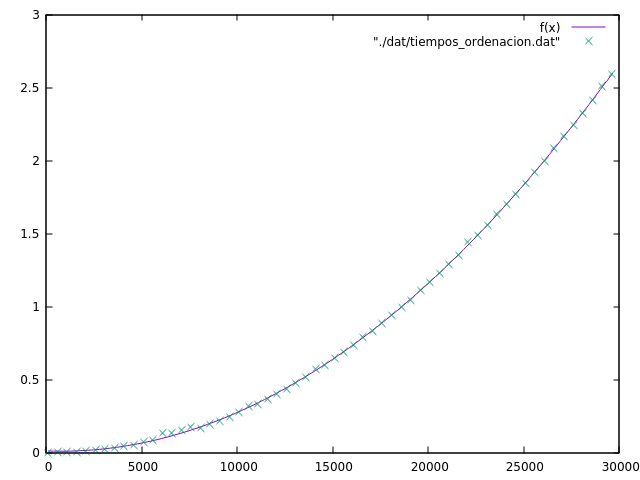
\includegraphics[width=0.5\textwidth]{./img/ef_pract_ej_2.png}
\end{figure}
\newpage
%Ejercicio 3
\textbf{\large Ejercicio 3.} Junto con este guión se le ha suministrado un fichero ejercicio\_desc.cpp. En él se ha implementado un algoritmo. Se pide que:\\ 
	\begin{itemize}  
	\item  Explique qué hace este algoritmo.
	\item  Calcule su eficiencia teórica. 
	\item Calcule su eficiencia empírica.
	\end{itemize}
Si visualiza la eficiencia empírica debería notar algo anormal. Explíquelo y proponga una solución. Compruebe que su solución es correcta. Una vez resuelto el problema realice la regresión para ajustar la curva teórica a la empírica.
\vspace {1em}	

\underline{\emph{Solución:}}\\
El algortimo \textit{operacion} busca en un vector la posición de un elemento concreto. Para ello, utiliza tres índices: inf, sup y med; además de un booleano que indica si se ha encontrado o no. Al principio, inf apunta al primer elemento del vector, sup al último y med al elemento central. Mientras inf sea menor que sup y no hayamos encontrado al elemento, entraremos en un bucle que asigna a med el elemento medio entre inf y sup y compara el elemento que se encuentra en dicha posición con el elemento buscado para, en caso de no encontrarlo, asignar a inf el elemento siguiente a med (si es menor que el elemento buscado) o a sup el anterior a med. Así, en las sucesivas iteraciones del bucle vamos comparando con el elemento que se encuentra en la mitad, en la mitad de la mitad, en la mitad de la mitad de la mitad,... Este es el algoritmo conocido como búsqueda binaria.\vspace{1em}

	\hspace*{1cm}1. int operacion(int *v, int n, int x, int inf, int sup) \{ \\
	\hspace*{1cm}2.\hspace*{2em}	int med;\\
	\hspace*{1cm}3.\hspace*{2em}	bool enc=false; \{ \\
	\hspace*{1cm}4.\hspace*{2em}	while ((inf$<$sup) \&\& (!enc)) \\
	\hspace*{1cm}5.\hspace*{4em}		med = (inf+sup)/2; \\
	\hspace*{1cm}6.\hspace*{4em}		if (v[med]==x) \\
	\hspace*{1cm}7.\hspace*{6em}			enc = true;\\
	\hspace*{1cm}8.\hspace*{4em}		else if (v[med] $<$ x) \\
	\hspace*{1cm}9.\hspace*{6em}			inf = med+1;\\
	\hspace*{1cm}10.\hspace*{4em}		else \\
	\hspace*{1cm}11.\hspace*{6em}			sup = med-1; \\
	\hspace*{1cm}12.\hspace*{2em}	\}\\
  	\hspace*{1cm}13.\hspace*{2em}	if (enc) \\
  	\hspace*{1cm}14.\hspace*{4em}		return med; \\
	\hspace*{1cm}15.\hspace*{2em}	else \\
	\hspace*{1cm}16.\hspace*{4em}		return -1; \\
	\hspace*{1cm}17. \} \\
	
	\underline{Eficiencia teórica:} \\
	Línea 2 y 3: 1 OE (declaración de variable).\\
	Línea 4: 3 OE (3 operaciones aritmético-lógicas).\\
	Línea 5: 3 OE (2 operaciones artimético-lógicas, 1 asignación).\\
	Líneas 6-11: 4 OE (aplicando la regla del máximo: 1 acceso a vector, 2 operaciones aritmético-lógicas, 1 asignación\\
	Líneas 13-17: 2 OE (1 operación aritmético-lógica, 1(return?))\\

	Al ser los otros bloques O(1) es, por tanto, el bucle de la línea 4 el que determina la eficiencia del algoritmo. Como los índices involucrados en la condición del mismo varían dividiendose entre dos, vamos quedándonos cada vez con menos elementos, de forma que la eficiencia es O(log2n). Concluimos, aplicando la regla de la suma, que la eficiencia de este algoritmo es O(log2n).\\
	
	\underline{Eficiencia empírica} \\
	Para calcular la eficiencia empírica creamos mediante /src/ejercicio\_desc.cpp el ejecutable /bin/ejercicio\_desc. El guión /csh/ejercicio\_desc.csh guarda en /dat/tiempos\_ejercicio\_desc.dat los tiempos de ejecución del programa con datos entre 100 y 1000000. Usando gnuplot, generamos la siguiente gráfica:
	
	\begin{figure}[!ht]
  \caption{Tiempos operacion}
  \centering
    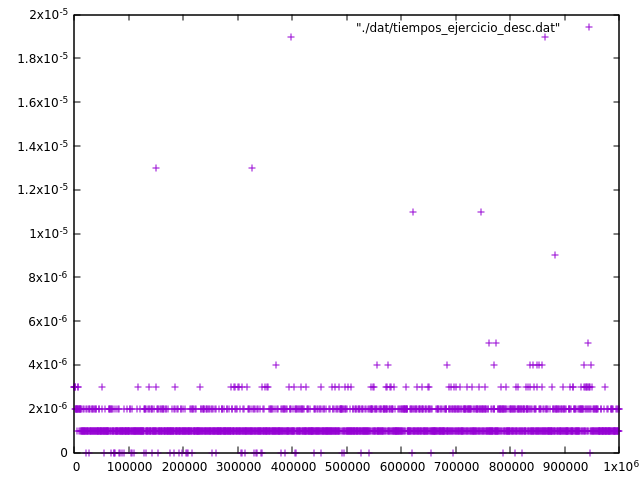
\includegraphics[width=0.5\textwidth]{./img/ef_pract_ej_3.png}
\end{figure}
	
	Observamos que esta gráfica no es logarítmica, como habíamos predicho de forma teórica, sino que los valores se mantienen en tiempos relativamente constantes. Esto se debe a que la precisión con que medimos los tiempos no es suficiente. Como solución se aporta el archivo /src/ejercicio\_desc\_sol.cpp. En él se realiza, para cada tamaño, 1000 veces \textit{operacion} y el tiempo tardado se divide entre 1000.
	Una vez realizada la regresión, observamos en la siguiente gráfica cómo queda la eficiencia teórica frente a la empírica:
	\begin{figure}[!ht]
  \caption{Comparación eficiencia teórica(f(x)), eficiencia práctica}
  \centering
    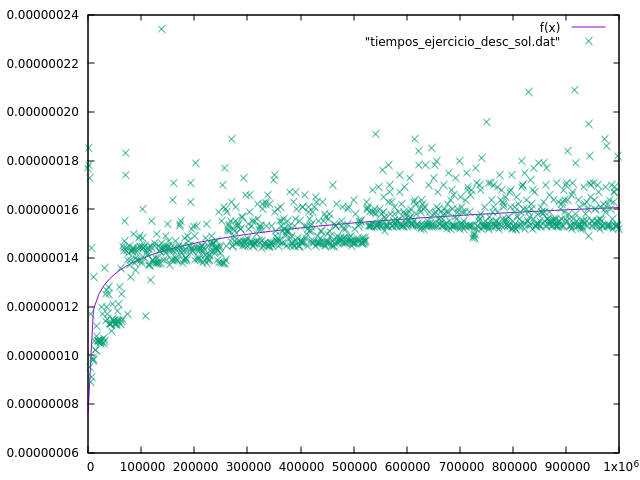
\includegraphics[width=0.5\textwidth]{./img/ef_pract_ej_3_2.png}
\end{figure}
\newpage
  
 %Ejercicio 4
	\textbf{\large Ejercicio 4.} Retome el ejercicio de ordenación mediante el algoritmo de la burbuja. Debe modificar el código que genera los datos de entrada para situarnos en dos escenarios diferentes:
	\begin{itemize}
	\item	El mejor caso posible. Para este algoritmo, si la entrada es un vector que ya está ordenado el tiempo de cómputo es menor ya que no tiene que intercambiar ningún elemento.
	\item	El peor caso posible. Si la entrada es un vector ordenado en orden inverso estaremos en la peor situación posible ya que en cada iteración del bucle interno hay que hacer un intercambio. 
	\end{itemize}
	Calcule la eficiencia empírica en ambos escenarios y compárela con el resultado del ejercicio 1.
\vspace {1em}	

\underline{\emph{Solución:}}\\
Como solución a este ejercicio creamos dos nuevos archivos .cpp que recogen ambos casos. A continuación, ofrecemos la gráfica en que se comparan los tiempos de ejecución de los tres casos:

\begin{figure}[!ht]
  \caption{Comparación ordenación normal/mejor caso/peor caso}
  \centering
    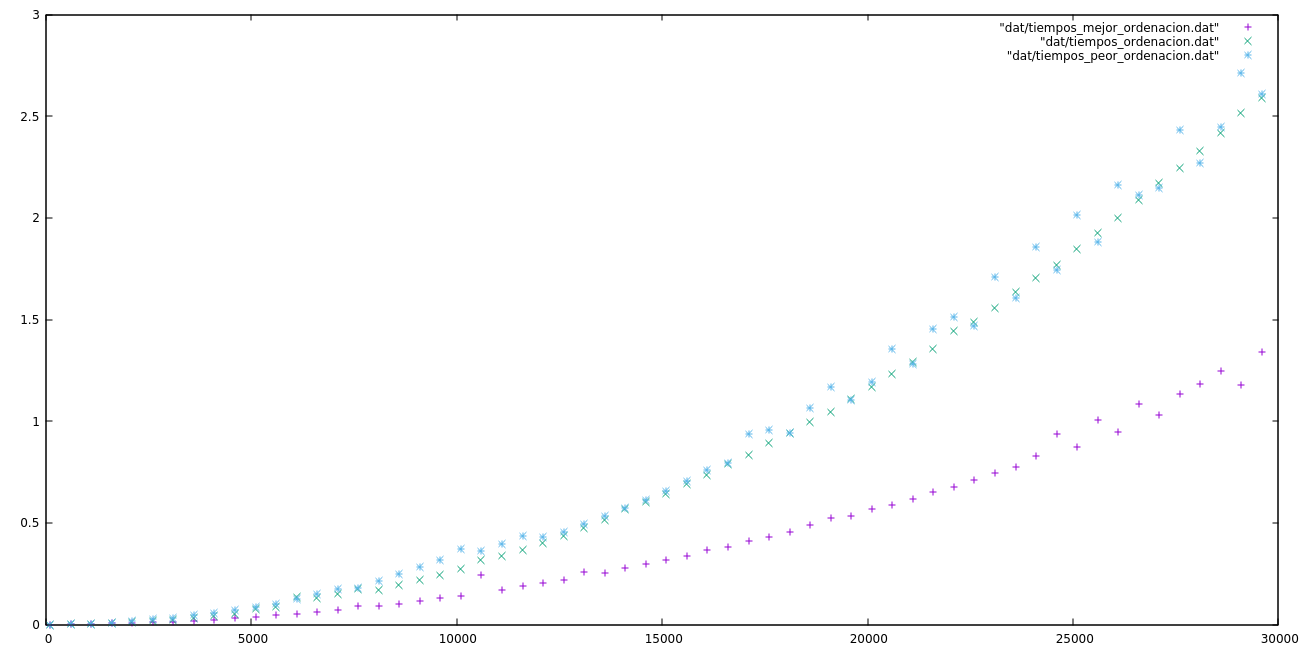
\includegraphics[width=0.5\textwidth]{./img/ef_pract_ej_4.png}
\end{figure}  

Se aprecia un menor tiempo de ejecución cuando el vector ya está ordenado frente a cuando está ordenado de forma inversa o desordenado de forma aleatoria.
\newpage

%Ejercicio 5
\ 
  \textbf{\large Ejercicio 5.} Dependencia de la implementación:\\ 
  
  \hspace*{1cm}1. void ordenar(int *v, int n) \{ \\
  \hspace*{1cm}2.\hspace*{2em}  bool cambio=true;\\
  \hspace*{1cm}3.\hspace*{2em} 	for (int i=0; i$<$n-1 \&\& cambio; i++) \{ \\
  \hspace*{1cm}4.\hspace*{4em}      cambio=false; \{\\
  \hspace*{1cm}5.\hspace*{4em}      for (int j=0; j$<$n-i-1; j++)\{ \\
  \hspace*{1cm}6.\hspace*{6em}        if (v[j]$>$v[j+1]) \{\\
  \hspace*{1cm}7.\hspace*{8em}        cambio=true;\\
  \hspace*{1cm}8.\hspace*{8em}		  int aux = v[j]; \\
  \hspace*{1cm}9.\hspace*{8em}		  v[j] = v[j+1]; \\
  \hspace*{1cm}10.\hspace*{7em}		  $\ $v[j+1] = aux; \\
  \hspace*{1cm}11.\hspace*{6em}\} \\
  \hspace*{1cm}12.\hspace*{4em}\} \\
  \hspace*{1cm}13.\hspace*{2em}\} \\
  \hspace*{1cm}14. \}  \vspace {1em} \\

En ella se ha introducido una variable que permite saber si, en una de las iteraciones del bucle externo no se ha modificado el vector. Si esto ocurre significa que ya está ordenado y no hay que continuar.\\\\
Considere ahora la situación del mejor caso posible en la que el vector de entrada ya está ordenado. ¿Cuál sería la eficiencia teórica en ese mejor caso? Muestre la gráfica con la eficiencia empírica y compruebe si se ajusta a la previsión.
\\

\underline{Cálculo eficiencia teórica:}
\\\\
En cada línea de código se producen las siguientes operaciones elementales:

Línea 2: 1 OE inicialización booleana\\
Línea 3: 4 OE inicial. "$\ $i ", comparación "$<$", resta "n-1", incremento "$\ $i++"\\
Línea 4: 1 OE asignación booleana\\
Línea 5: 5 OE inicial. "j", comp. "$<$", doble resta "n-i-1", incremento "j++"\\\\
Línea 6: 4 OE accesos a v[j] y v[j+1], suma "j+1", comp. "$>$"\\
Línea 7: 1 OE asign. bool.\\
Línea 8: 2 OE inicial. "$\ $aux", acceso a v[j]\\
Línea 9: 4 OE acceso a v[j] y v[j+1], suma "j+1", asignación\\
Línea 10: 3 OE acceso a v[j+1], suma "j+1", asignación\\

*Las líneas 7-10 no sucederían en el mejor de los casos, cuando el vector está ordenado
\ 
\\\\ 
Por tanto, en el mejor de los casos, donde el primer bucle sólo produce una iteración:\\ 
$$T(n)=1\ +\ 1\ +\sum \limits_{j=0}^{n-1} 4= 1+1+(\frac{4+4}{2})\cdot(n-1)= 4n-2 $$\newpage
\underline{Eficiencia práctica:}\\

\begin{figure}[!ht]
  \caption{Gráfica eficiencia práctica}
  \centering
    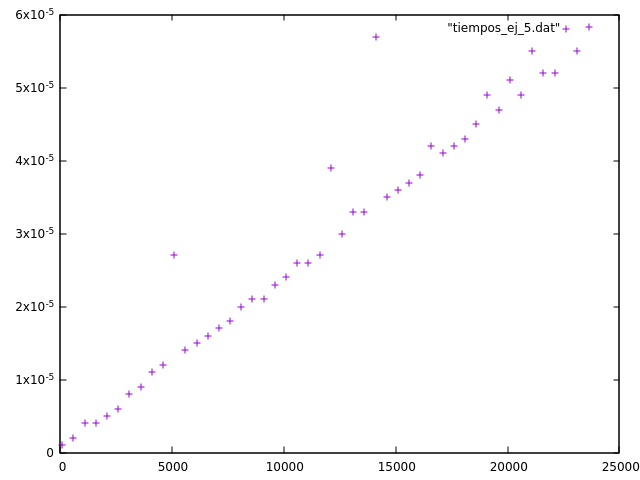
\includegraphics[width=0.5\textwidth]{./img/ef_pract_ej_5.png}
\end{figure}

\newpage
%Ejercicio 6

\textbf{\large Ejercicio 6.} Influencia del proceso de compilación:\\

Retome el ejercicio de ordenación mediante el algoritmo de la burbuja. Ahora replique
dicho ejercicio pero previamente deberá compilar el programa indicándole al compilador
que optimice el código. Esto se consigue así:
$$g++\ -O3\ ordenacion.cpp\ -o\ ordenacion\_optimizado$$
\\
Compare las curvas de eficiencia empírica para ver cómo mejora esto la eficiencia del
programa.
\\


\begin{figure}[!ht]
  \caption{Comparación ordenación normal/optimizado}
  \centering
    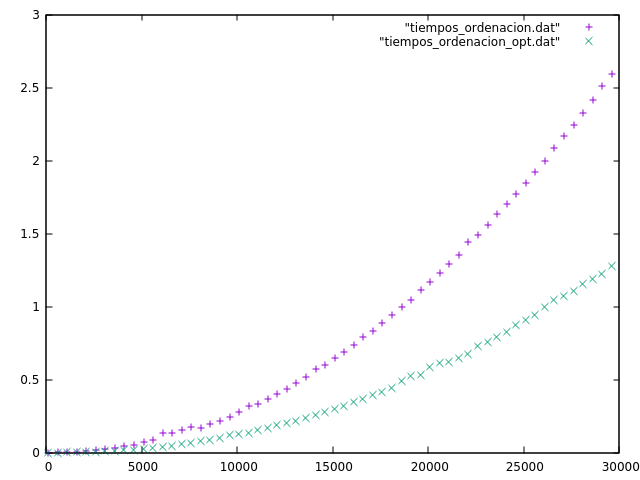
\includegraphics[width=0.5\textwidth]{./img/ef_pract_ej_6.png}
\end{figure}
 
\vspace {1em}  	


\end{document}
